\documentclass{article}
\usepackage[utf8]{inputenc}
%---------------------------------------------------------------------------------------
%	TITLE HEADLINE
%----------------------------------------------------------------------------------------
\vspace{-3pt}
% use this for multiple words like working titles etc.
%\hspace{-0.25\linewidth}\colorbox{bgcol}{\makebox[1.5\linewidth][c]{\hspace{46pt}\HUGE{\textcolor{white}{\uppercase{M.Sc. Jan Küster}} } \textcolor{sectcol}{\rule[-1mm]{1mm}{0.9cm}} \parbox[b]{5cm}{   \large{ \textcolor{white}{{IT Consultant}}}\\
% \large{ \textcolor{white}{{JS Fullstack Engineer}}}}
%}}
% use this for single words, e.g. CV or RESUME etc.
\colorbox{darkcol}{\makebox[\mpwidth][c]{\HUGE{\textcolor{lightcol}{\uppercase{Alan Matzumiya}} } }}

%----------------------------------------------------------------------------------------
%	HEADER IMAGE
%----------------------------------------------------------------------------------------

%\includegraphics[trim= 0 250 0 270,clip,width=1\linewidth+3.1cm]{myfoto.jpg}	%trimming relative to image size!

\includegraphics[width=0.9995\linewidth]{../../img/formal-banner.png}	%trimming relative to image size

%---------------------------------------------------------------------------------------
%	SUMMARY
%----------------------------------------------------------------------------------------
\transparent{0.85}%
\vspace{-127pt}
\hspace{0.32\linewidth}
\colorbox{darkcol}{
    \parbox{0.60\linewidth}{\vspace{-1.15mm}\hspace{-2.10mm}\colorbox{fgreycol}{\parbox{1.025\linewidth}{\textcolor{lightcol}{\hspace{0.22\linewidth}Alan Daniel Matzumiya Zazueta}}}
        \vspace{-4.5mm}
        \transparent{1}%
        \begin{center}
            \larrow{softcol}\larrow{softcol}\larrow{softcol} \textcolor{lightcol}{Soy Ingeniero Qu\'imico y Maestro en Ciencias Matem\'aticas. Adem\'as, Cuento con Fuertes Conocimientos en Desarrollo de Software / Web}
        \end{center} 
    }
}
\vspace{50.5pt}
\transparent{1}%

%  \usepackage{refcheck}


\topmargin-4mm\textheight230mm\oddsidemargin4mm\evensidemargin5mm \textwidth165mm \parindent0mm\marginparsep3mm\marginparwidth30mm

%\topmargin-4mm\textheight230mm\oddsidemargin4mm\evensidemargin5mm \textwidth150mm \parindent0mm\marginparsep3mm\marginparwidth30mm


%opening
\title{\vspace*{-3cm}\large\bf {\rm Anteproyecto de investigaci\'on}\\
Kolmogorov equations associated to Stochastic partial differential equations:  Numerical methods, Applications and related topics.}

 
\author{{\bf Alumno: Alan Daniel Matzumiya Zazueta}\\
Comit\'e Tutoral  :  Dr. Francisco Delgado-Vences. (Supervisor de tesis)\\
\hspace*{-.9cm} Dr. Luis Antonio Rinc\'on Sol\'{i}s\\
\hspace*{-.9cm} Dr. Fernando Baltazar Larios
}

\numberwithin{equation}{section}

\RequirePackage[OT1]{fontenc}
\RequirePackage{amsthm,amsmath,amssymb,mathtools}
\RequirePackage[colorlinks,citecolor=blue,urlcolor=blue]{hyperref}


\date{}
\begin{document}

\maketitle
%\tableofcontents

\section{Antecedentes}
The project relies on Kolmogorov equations associated to Stochastic partial differential equations (SPDE's) and some related topics, in particular, on numerical methods for Kolmogorov equations and applications of SPDEs to several fields of knowledge. \\

The study of Stochastic Partial Differential Equations is an interdisciplinary area at the crossroads of stochastic processes, functional analysis and partial differential equations. In this project, we will add to this mixture two more areas of mathematics: numerical analysis and inverse problems.
SPDE's are an important tool for increasing our understanding of basic (physical, chemical, biological, economic, finance,
etc.) processes, and can play a central role in uncertainty quantification and risk assessment, for
instance see \cite{le-kn}. \\

A Stochastic Differential Equation (SDE) is an ordinary differential equation in which one or more of its terms is a
stochastic process and whose solution is also a stochastic process. SDEs are used to model
random fluctuations that cannot be adequately represent by an Ordinary Differential Equation (ODE).
Thus,  SDE's are a kind of generalization of ODE's (see \cite{ok}).\\


Stochastic partial differential equations (SPDE's) generalize partial differential equations (PDE) via random forces 
and random coefficients, in the same way that SDEs generalize ODEs. However, this generalization is more tricky and highly technical than the one for ODEs.\\ 


There are several approaches to study SPDE's, one of them are those whose solution take values in Hilbert spaces and that are driven by a cylindrical Wiener process or a colored noise in space and white in time (see \cite{da-za1}, \cite{lo-ro}, \cite{lo-ro-06}). 
In addition, one could study Kolmogorov equations associated to SPDE's (see \cite{da-za},\cite{da}, \cite{da1}).
These latter equations are diffusions on infinite dimensional separable Hilbert spaces, these equations are deterministic PDEs that by themselves are ver interesting to study and develop theory about it. \\



It is well-known that SDEs and SPDEs, are very important to study several phenomena that appears in Financial mathematics, (see for instance 
Carmona \cite{ca}) or in Biology \cite{le-pe-po}, so we are interested on applications of these models to problems in these two field of knowledge. However, the knowledge of several properties of solutions of SDEs and SPDEs are crucial when one want to study and model using it. Moreover, in order to appy these models it is important to develop numerical and statistical properties of the SDEs and SPDEs.\\


% Malliavin Calculus is a calculus for functionals of stochastic processes, moreover, it allows to define a derivative into the probability space, this is obtained with the use of functional analysis. The Malliavin calculus allows integration by parts with random variables; this operation is used in mathematical finance to compute the sensitivities of financial derivatives. See for further reading Nualart \cite{nu} or Nualart and Nualart \cite{nu-nu}.\\

 
Francisco Delgado and Franco Flandoli have introduced a spectral numerical method for Kolmogorov equations that is very helpful to study 
several properties of the related SPDE's, moreover, with this numerical method it is also possible to study deterministic partial differential equation 
related to the SPDE. Inded, 
the numerical method introduced in \cite{de-fl} to study Kolmogorov (FPK) equations associated with SPDEs in separable Hilbert spaces allows us to simulate in an efficiente the mentionated SPDEs. This is very important in forward problems. Furthermore, In these project, within the following two years, we will study an inverse problem for SPDEs using a spectral representation of the solution of a SPDE in a Hilbert space. This could help us to estimate parameters and even more, to approximate nonlinear functions of the solution of SPDEs and then to study nonlinear problems that could appear in fields such as, physics, biology, economics, finance, etc. \\



I now present in detailed the topics we will work on my Ph.D. studies.

 \section{Numerical method for Kolmogorov equations associated with SPDE's in Hilbert spaces} 
 The development of efficient numerical analysis and its
implementation for the solution of SPDE's has become a very active area of research, which is not surprising since the use of SPDE's in mathematics as well as in other fields of science has strongly increased in the last decades. However, numerical methods for FPK equations have been understudied, probably due to the complexity they represent.\\
 
One of the main advantages of FPK equations lies in the fact that the joint Probability Density Function (PDF) of the response of the
nonlinear system can be directly obtained by using these kinds of equations, and then several statistics
and quantities of interest of the solution such as the first passage time and level crossing statistics can
be obtained from the joint PDF. The proposed project will provide a method to simulate and get
information efficiently and directly. Moreover, the FPK equation provides a very useful tool for
modeling a wide variety of stochastic phenomena arising in physics, chemistry, biology, finance,
traffic flow, etc. Furthermore, several kinds of stochastic differential equations, partial or ordinary,
can be linked to an FPK equation. Thus, developing a good method for the numerical solution of the
FPK equation is important to study several phenomena in nature, finance, engineering, etc.\\

In Delgado and Flandoli \cite{de-fl}, it was introduced a numerical method to solve FPK equations and tested this
method by applying it to the Kolmogorov equations associated with two stochastic partial differential
equations: a stochastic diffusion and a stochastic Burgers equation in 1D, both in a simple domain. The
proposed numerical method is based on the spectral decomposition of the Ornstein-Uhlenbeck
semigroup associated with the Kolmogorov equation. This decomposition is used to reformulate the
Kolmogorov equation as an infinite system of ordinary differential equations, and by truncating it we
obtain a finite coupled linear system of differential equations. The solution of such system allows us to
build an approximation to the solution of the Kolmogorov equation. The Fokker-Planck-
Kolmogorov (FPK) equations associated with stochastic partial differential equations
is a deterministic, but infinite dimensional, partial differential equation, that describes
the time evolution of the PDF of the velocity of a particle under the influence
of drag forces and random forces; it is a kind of continuity equation for densities.\\

\subsection{A brief description of the numerical method for Kolmogorov equations}\label{num-kol-sect}
Following Delgado-Flandoli \cite{de-fl}, we consider the following SPDE. 
Set a separable Hilbert Space $\mathcal{H}$  and consider the SDE in $\mathcal{H}$
\begin{align}
 dX_t&=\gamma AX_tdt+B(X_t)dt+\sqrt{Q}dW(t),\label{P1s2.1}\\
X(0)&=x, \qquad x\in\mathcal{H},\nonumber
\end{align}
where  $A:\mathcal{D}(A)\subset \mathcal{H}\rightarrow \mathcal{H}$ is an  operator, $Q$ is another bounded operator from (possibly) another
Hilbert space $\mathcal{U}$ to $\mathcal{H}$ and $B:\mathcal{D}(B)\subset \mathcal{H}\rightarrow \mathcal{H}$ is a nonlinear mapping. 
$W$ is a cylindrical Wiener process on $\mathcal{U}$. Here $\gamma$ is a parameter.

The solution to \eqref{P1s2.1} is given by
\begin{equation}\label{s2.2}
 X(t,x)=e^{tA}x + \int_0^t e^{(t-s)A}B(X_s) ds  +  \int_0^t e^{(t-s)A}\sqrt{Q}dW(s),\qquad t\ge 0.
\end{equation}
where, the last integral is a stochastic integral in the Hilbert space $\mathcal{H}$ and $e^{tA}$ is the $C_0$-semigroup generated by $A$.
 
 Formally, the cylindrical Wiener process $W(t)$ can be written as the series
 \begin{equation}
  W(t)=\sum_{k=1}^\infty \beta_k(t) e_k,
 \end{equation}
where the sum converges in $L^2$ sense, $\{e_k\}$ is an orthonormal basis for the Hilbert space $\mathcal{H}$ and $\beta_k(\cdot)$, $k\in\IN$ 
are mutually independent Brownian motions.

We formally write the stochastic integral as the convergent (in $L^2$) series
\begin{equation}
\int_0^t e^{(t-s)A}\sqrt{Q}dW(s)=\sum_{k=1}^\infty \int_0^t e^{(t-s)A}\sqrt{Q}e_kd\beta_k(s),
 \end{equation}
where 
\begin{equation}
\int_0^t e^{(t-s)A}\sqrt{Q}e_kd\beta_k(s) = \sum_{i=1}^\infty \int_0^t \langle e^{(t-s)A}\sqrt{Q}e_k,e_i\rangle_{\mathcal{H}} d\beta_k(s)\hspace*{0.05cm} e_i. 
 \end{equation}

With all these ingredients it is well-known that the existence and uniqueness of a mild solution for \eqref{P1s2.1} $X$ is given 
by \eqref{s2.2}(see \cite{da-za1} for instance). We proposed a numerical weak approximation to the solution $X$ trough the Kolmogorov
equation. Define $u(t,x)=\E[u_0(X_t^x) ] $, where $u_0:\mathcal{H}\rightarrow \IR$ is a linear functional and $X_t^x$ 
is the solution to \eqref{P1s2.1} with initial conditions $X_0=x$, $x\in\mathcal{H}$.  Then $u$ satisfies the 
{\bf Kolmogorov equation}  (see \cite{da-za} for instance):
\begin{equation}
\label{P1s2.3}
\frac{\partial u}{\partial t}= \frac{1}{2}Tr(QD^2u)+ \langle Ax, Du \rangle_\mathcal{H} + \langle B(x),Du \rangle_\mathcal{H},\quad x\in D(A).
\end{equation} 
This is a deterministic PDE but infinite dimensional since $x\in \mathcal{H}$. Then, by using several results it is possible to 
decompose the space $\mathbb{H}:=L^2( \mathcal{H},\mu)$ as an infinite direct sum of closed subspaces:
 \[
\mathbb{H} = \bigoplus_{j=0}^\infty K_j,
\]
and with this decomposition we can write the solution $u$ of the Kolmogorov equation as a Fourier-Hermite series:
\begin{equation}
\label{s3.1}
u(t,x) =  \sum_{\bar{n}\in \mathcal{J}} u_{\bar{n}}(t) H_{\bar{n}}(x), \qquad x\in\mathcal{H},\quad t\in[0,T].
\end{equation}
Here it is important to mention that this decomposition is not trivial and is a deterministic version 
of the Wiener-Hermite chaos expansion (see for instance \cite{lo-ro} for further reading).
With this decomposition  we can fix an infinite linear coupled system of ODE's to estimate each $u_{\bar{n}}(t)$. By truncation of 
the series \eqref{s3.1} we obtain an approximation to the Kolmogorov equation which is a weak approximation to 
the SPDE \eqref{P1s2.1}.




\subsection{Continuity of the initial conditions}
 As a first result, in collaboration
with F. Delgado-Vences and S. Diaz-Infante, we are concluding the 
study of the continuity of the initial conditions for the numerical method descrided in section \ref{num-kol-sect}. This is important when one wants to prove that the initial
value problem (IVP) is well possed. In our case, the IVP is an infinite dimensional PDE and we prove that both, the analytical solution and 
the numerical solution, are continuous with respect to the initial conditions. We have proved results such as
\begin{align*}
\|  u(t,\varphi)-u(t,\psi)\|_{\mathbb{H} } &\le \exp(Ct)  \|  \varphi - \psi\|_\mathcal{H} 
\end{align*}
which implies continuity with respect to the initial conditions. We have writen a research paper that has been submitted to a peer-reviewed journal.

\section{Problemas propuestos}
\subsection{Numerical approximation to the stochastic Navier-Stokes equations in $d=2$}
 The first project to work  is related to the application of the numerical method for the Kolmogorov equation associated with the 
stochastic Navier-Stokes equations in dimension 2. We will use this numerical method to construct a weak approximation to the 
stochastic Navier-Stokes equations and we will try to obtain a rate of convergence for this approximation.
This is a project in collaboration with Francisco Delgado and Hakima Bessaih. 


Set $\mathcal{O}:=\R\times (0,1)$, $X=(X_1,X_2)$, $\xi=(\xi_1,\xi_2)$.\\
 Consider the stochastic equation in $\mathcal{O}$
 \begin{align*}
&d X=\Big[ \gamma \Delta X - (X\cdot \triangledown)X + \triangledown P\Big]dt+\sqrt{Q}dW(t),\\
&div\hspace*{0.1cm} X=0,\qquad \xi\in\mathcal{O}, t\ge 0.\nonumber\\
%&\partial_{\xi_2}X_1(t,\xi_1,0)=\partial_{\xi_2}X_1(t,\xi_1,1)=0,\qquad t\ge 0, \xi_1\in\R\\
%&X_2(t,\xi_1,0)=X_2(t,\xi_1,1)=0,\qquad t\ge 0, \xi_1\in\R\\
%&X(t,\xi_1+L,\xi_2)=X_2(t,\xi_1,\xi_2)\qquad t\ge 0, (\xi_1,\xi_2)\in \mathcal{O}\\
&X(0,\xi)=x(\xi), \qquad\xi\in \mathcal{O}.
\end{align*}
 $X=(X_1,X_2)$ is the velocity field and $W$ is a cylindrical Wiener process on some Hilbert space.
 
  
  \begin{figure}[H]
 \begin{center}
 
 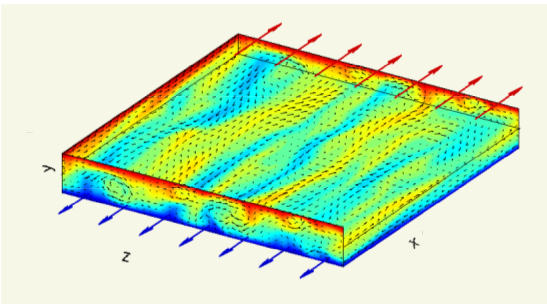
\includegraphics[width = 1.95in]{u-box.jpeg} 
 %\caption{Simulations for the Burgers equation with the Matlab library {\it pdepe} and with
% the spectral method for $N=4,5$, $u_0^{\xi_0}(g)=g(\xi_0)$.}
 \label{graph-simu_nu4.1}

 \end{center}
\end{figure}
We will use the vorticity formulation and we will use the numerical scheme for the Kolmogorov equation,
developed in \cite{de-fl}, to get estimates for the weak approximation of the SPDE. 




\subsection{A numerical comparison between strong and weak approximations to solutions of SPDEs}

 The numerical strong approximations is based on the well-known Wiener-Chaos expansion (see for instance \cite{lo-ro} or \cite{ka-zh} and the references therein) and it is a kind of Fourier expansion of the solution. However, this Fourier expansion is defined in the probability space that is usually taken as a suitable subspace of an infinite dimensional Banach space. The usual procedure is the following. One takes a family of suitable polynomial $\Psi_n(\cdot)$ and a sequence of independent random variables $\xi_1,\ldots,\xi_m$. Next, in order to built the Fourier expansion, we need to fix the coefficients of the Fourier expansion, here it is necessary to evaluate the sequence of random variables in each polynomial, i.e.,
 \begin{equation}
  u(t,x) \approx u^{n,m}(t,x):=\sum_{(j,k)=(1,1)}^{n,m} u_{j,k}(t,x) \Psi_j(\xi_k)
 \end{equation}
 
 
It is well-know that the strong approximation has the so-called {\it curse of dimensionality} problem: It is necessary to fix  a high number of coefficients to set up the approximation. There exists several manners to try to overcome this difficult to obtain optimized simulations and sometimes it is successfuly. However, when the SPDEs that one try to solve numerically is strongly nonlinear then it is necessary to implement the numerical approximation using families of polynomials $\Psi_n(\cdot)$ not so simples, for instance, product of Hermite polynomials and in such case the number of coefficients is even higher (see \cite{ka-zh}) .
 
The numerical approximations introduced by Delgado-Vences and Flandoli is a weak approximations that has shown be free of the {\it curse of dimensionality}, the main difference between the two approximations is that in the weak approximation one have to estimate or adjust a very small number of coefficients, this is doubt to the fact that the weak approximations uses a nice spectral representation of the solution. Indeed, taking a basis for a Hilbert space continuously embedded in the Banach space that is the probability space, then one have that such basis now played the role of the  sequence of random variables $\xi_1,\ldots,\xi_m$ and will reduced the problem of fix to many coefficients.

In this part of the project we will work on a comparison of this two types of numerical approximations.

\subsection{A microlocal spectral method for PDEs by noise}\label{microlocal}


In opposition to the last subsections, here we will start with a Partial Differential Equation and we will add some suitable noise in such way that we have a SPDE like Equation \eqref{P1s2.1}. We will consider that the PDE and the SPDE has a mild solution such as in \eqref{s2.2}. We then, now will pass to the Kolmogorov equation and we will solve numerically the Kolmogorov equation, the last part means that we will solve an equation for the mean of a given functional of the solution of the SPDE. Therefore, we could come back and solve numerically the PDE with an spectral method that has the property of get a spectral representation of the solution point by point, we strongly believed that this could help us to propose spectral-based numerical solutions to PDEs with {\it discontinuous} initial conditions.

\subsection{ Weak approximations of SPDE's}
Another project is the study of weak approximations of SPDE's by using the numerical approximation of the Kolmogorov equations proposed in \cite{de-fl}. It is well-known that it is tipically more complicated to prove the weak approximation of SPDE's than it is to prove  the strong 
approximation. It seems that the numerical method proposed by Delgado-Vences and Fladoli have good enough properties to prove the weak 
approximations in a easier way that with other methods (see for instance \cite{deb1} or \cite{de-pr}). We will use several ideas from data 
assimilation to prove this types of results. This is a project in collaboration with 
Hakima Bessaih. 


\subsection{Inverse problems for stochastic and deterministic PDEs.}

Focus again on the Equation \eqref{P1s2.1}, in particular on the parameter $\gamma$ . Depending on the context of the equation $\gamma$ should represent different properties of the enviroment, for instance sometimes is the thermal diffusivity, the viscosity coefficient, etc. In this part of the project we will assume that the parameter $\gamma$ is unknown and we will propose a feasible numerical method to estimate $\gamma$. There exists in literature several inference methods for estimating this type of parameters, however its practical applicability has not been tested and we consider is not adequate to work with real problems.

The idea is the following. Consider the Kolmogorov equation associated to  Equation \eqref{P1s2.1}, it means \eqref{P1s2.3} and its numerical approximation \eqref{s3.1}. Since, we are working on a Hilbert space continuously embedded in the infinite dimensional Banach space then we are, actually, working on an {\it abstract Wiener space}. Therefore, we can take as a functional  $u_0:\mathcal{H}\rightarrow \IR$ the evaluation functional for some $\xi_1,\ldots,\xi_m$. Afterward, we can define $m$ SPDEs that will describe the evolution of each $X_t^x(\xi_j)$, $j=1,\ldots,m$ and we approximate each of these equations in the following sense
\begin{align}
 u^N(t,x,\xi_j)\approx u(t,x,\xi_j)=\E\big(X_t^x(\xi_j) \big)
\end{align}

Then we will propose an estimator for $\gamma$ as follows
\begin{align}
 \hat\gamma := \arg\min_{\gamma} \sum_{j=1}^m\int_0^t \Big| u^N(s,x,\xi_j)-\E\big(X_s^x(\xi_j) \big) \Big|_{\mathcal{H}}^2  ds
\end{align}


We first will test the proposal estimator with the help of simulations. A posterior step will be get data and apply the method. Notice that given the discussion in Section \ref{microlocal} the same estimator $ \hat\gamma $ will serve for PDEs.




\subsection{Applications of stochastic (partial) differential equations.}

We want to study applications of stochastic (partial) differential equations to several fields of science. In particular, we are interested on Ecology, Financial mathematics and Vulcanology. In Ecology we could be able to get data to apply SPDES during the first year of the PhD, while in finances we will look for it. Here we describe two of the project we have concrete ideas. 

\begin{itemize}


\item In the medium term, I plan to start with a model for the behavior of magma fluid inside the magma chamber of a volcano. We want to apply the numerical simulation for the stochastic Navier-Stokes equations that we are developing with Hakima Bessaih. However, given that  magma behaves like a non-newtonian fluid, it is necessary to develop a stochastic model that could cover this case. Our main idea is to consider the stochastic Navier-Stokes equations with a generalized newtonian fluids. This will imply that the extension and application of the model is not trivial and will require good knowledge of the stochastic model and the numerical  method to solve the stochastic Navier-Stokes with a generalized newtonian fluid. This project will be develop in 
collaboration with Simone Colucci from the INGV- Pisa, Italia, and possibly other researchers.

 \begin{figure}[H]
 \begin{center}
 
 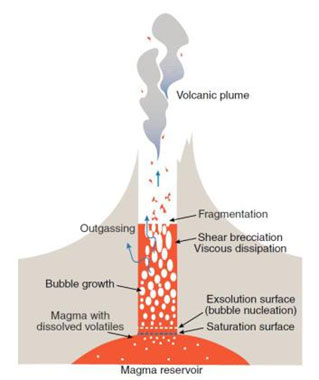
\includegraphics[width = 2.95in]{carrico2.jpg} 
 %\caption{Simulations for the Burgers equation with the Matlab library {\it pdepe} and with
% the spectral method for $N=4,5$, $u_0^{\xi_0}(g)=g(\xi_0)$.}
 \label{graph-simu_nu4.1}

 \end{center}
\end{figure}


\item A subsequent work will be to develop a tochastic model for volcanic ash transport and dispersal. As before we are interested in applying the stochastic Navier-Stokes equations with a generalized newtonian fluid but also in using a different approach, the Smoluchowski Diffusion equation. The Smoluchowski equation is a system of partial differential equations modeling the diffusion and binary coagulation of a large collection of tiny particles. It is well known that the 
Smoluchowski equation is the Fokker–Planck equation for the probability density function of the particle positions of 
Brownian particles. At this point we could try both approaches to model volcanic ash transport and dispersal with these two stochastic models and 
adapt the numerical method for Kolmogorov equations already proposed in \cite{de-fl}. This project will be developed in collaboration
with Arnau Folch from the Barcelona Supercomputing Center.

\end{itemize}


\vspace*{-0.2cm}
%\section*{Referencias}
\begin{thebibliography}{99}


\bibitem{ca} (R. Carmona and M. Tehranchi: {\it Interest Rate Models: an Infinite Dimensional Stochastic Analysis Perspective}. Springer Verlag (2006)

\bibitem{da} G. Da Prato : Kolmogorov equations for stochastic partial differential equations.
Advanced Courses in Mathematics - CRM Barcelona. Birkh\"auser. (2004).
 
 \bibitem{da-za} G. Da Prato, J. Zabczyk : Second order partial differential equations in Hilbert spaces.
 Cambridge University Press, (2002).

 \bibitem{da-za1} G. Da Prato, J. Zabczyk: Stochastic equations in infinite dimensions.
Cambridge University Press, second edition (2014).

\bibitem{da1} G. Da Prato: An introduction to Kolmogorov equations in Hibert spaces. Lecture notes. May 2011. (2011).

\bibitem{deb1} A. Debussche: {\it Weak approximation of stochastic partial differential equations: the nonlinear case}, Math of Comp, 80, 
pp. 89-117 (2011).

\bibitem{de-pr} A. Debussche, J. Printems: {\it Weak order for the discretization of the stochastic heat equation},
Math of Comp, 78, 266, pp. 845-863 (2009).

\bibitem{de-fl} F. Delgado-Vences  and F. Flandoli :{\it A spectral-based numerical method for Kolmogorov equations in Hilbert spaces},  Infinite Dimensional Analysis, Quantum Probability and Related Topics, vol. 19, No. 3. (2016)

\bibitem{ka-zh} G. Karniadakis, Z. Zhang : Numerical methods for stochastic partial differential equations with white noise
 Springer. (2017)

\bibitem{le-kn}  O.P. Le Ma\'itre and  O.M. Knio: Spectral Methods for Uncertainty
Quantification, With Applications to Fluid Dynamics.
Springer, Berlin (2010)

\bibitem{le-pe-po} M. A. Lewis, S. V. Petrovskii, J. R. Potts: The Mathematics Behind Biological Invasions. 
 Springer International Publishing Switzerland (2016)
 
\bibitem{lo} S. V. Lototsky: {\it Statistical Inference for Stochastic Parabolic Equations: A Spectral Approach}. Publ. Mat. 
(Publicacions Matematiques), Vol. 53, No. 1, pp. 3–45, (2009).

\bibitem{lo-ro-06} S. V. Lototsky and B. L. Rozovskii: {\it Stochastic Differential Equations: A Wiener Chaos Approach}. 
In: Yu. Kabanov, R. Liptser, and J. Stoyanov (editors),
From Stochastic Calculus to Mathematical Finance: The Shiryaev Festschrift, pp. 433-507, Springer, 2006.

\bibitem{lo-ro} S. V. Lototsky and B. L. Rozovsky. Stochastic Partial Differential Equations. Springer, 2017.
% 
% \bibitem{mi-mo}  A. Millet, P.L. Morien, {\it On a nonlinear stochastic wave equation in the plane: existence and uniqueness of the solution}
% The Annals of Applied Probability.  Vol. 11, No. 3, 922–951. (2001)


% \bibitem{NP} I. Nourdin and G. Peccati: Normal approximations with Malliavin calculus. 
% From Stein's method to universality. Cambridge Tracts in Mathematics, 192. {\it Cambridge University Press}, Cambridge, 2012. xiv+239 pp.
% 
% \bibitem{nu} 
% D. Nualart: The Malliavin calculus and related topics. 
% Second edition. Probability and its Applications (New York). {\it Springer-Verlag, Berlin,} 2006. xiv+382 pp. 
% 
% \bibitem{nu-nu}
% D. Nualart  and E.  Nualart:  \emph{Introduction to Malliavin Calculus}. IMS Textbooks, Cambridge University Press, 2018.


\bibitem{ok} B. Oksendal, Stochastic Differential Equations, An Introduction with Applications. Springer. (2003)

% \bibitem{st-va} D. W. Stroock and S. R. S. Varadhan: Multidimensional Diffusion Processes. Springer Verlag, Berlin, (1979).
% Germany

\end{thebibliography}

\end{document}
